\section{Results}

Without any partitioning operation, the inner and outer boundary of of a shell model needs to be filled by a huge amount of support materials in order to guarantee a fine surface quality. See Figure \ref{fig:dear-simulation} (a-b) for an illustration of a deer model, both its inner and outer surface requires some amount of support in order not to be collapsed during the printing process; while our approach only keeps all cylinder-like shells that are free of support (Figure \ref{fig:dear-simulation} (c-d)).

\begin{figure}[tbp]
  \centering
  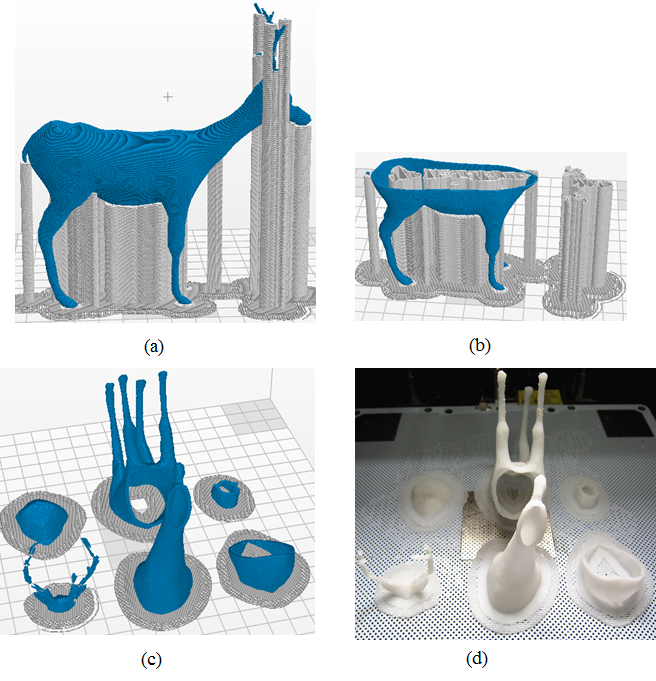
\includegraphics[width=\linewidth]{figs/dear-simulation.png}
  \caption{\label{fig:dear-simulation}%
           An illustration of a deer model under the 3D printing software Z-suite as the support angle is no larger than 20 degrees; (a) the full model; (b) an intermediate step of the simulation; (c) the simulation result of our partitioned shell models; (d) the 3D printed shell models free of support.}
\end{figure}


The following table summarizes the printing material and time costs by the original models and the partitioned models. The experiments are based on the choice of $\theta$ = 70 degrees.


Figure \ref{fig:partition} shows the effect of the partitioned models with our proposed approach, the printing direction of each part is orthogonal to its base (shown in the same color as the part). Figure \ref{fig:comparison} shows the comparison of the printing effects of the original models and our partitioned models. Note that the comparison of total cutting length cannot be made since no previous support-free oriented algorithms are available for 3D printed shell models.




[show the printed model without using any cutting operation, the partitioned CAD model, the assembled printed model, the statistics on time and material saving, for all 12 models]

Although the FDM based printing technique requires a small supporting bed for holding the printed model on the printing platform, other printing techniques such as SLA, SLM and SLS may avoid the use of these supporting beds. Therefore, our approach guarantees support-free to the most extent for all exiting printing techniques.

\hl {[Evaluations: how close we are to the global optimum]

[Limitations: discussion about 1. the strength of our interior, -- future work. 2. cut through salient regions -- hard to balance. etc] }

However, our approach suffers from a few limitations: for shell models, the thickness of the shells need to be large enough such that no serious deformation is caused during the assembling process. However, the problem of setting the thickness of the model in different parts of the model has not been investigated, our work only allows a uniform setting of the shell thickness whose value was determined by an error-and-trial process.

Finally, we propose a possible direction of future research. For 3D printing, the base should be flat in order to guarantee the support-free requirement, therefore it is difficult to cut the model through salient regions. However, a balance between the two may be achieved if slight relaxation of the support-free constraint is allowed, i.e., trading a subtle amount of support material with a round cut passing through salient regions may result in less amount of cuts and cutting length, and a better appearance on the assembled model.
